\documentclass[10pt,a4paper,twocolumn]{article}

\input{pisika.dat}
\usepackage{amsmath, bm, booktabs, caption, dcolumn, fancyhdr, geometry, graphicx, hyperref, latexsym, natbib}
%  Editorial staff will uncomment the next line
% \input{staff.hed}
\usepackage{float}
\author{ A travelling snail}
\title{   Mpemba effect  }
\begin{document}
	\maketitle
	\section{ Classical Mpemba effect}
	when we put two glasses of hot water and cold water into the same refrigerator,you may find the hotter one will freeze with less time.That is ridiculous.How can one state far from equilibrium state reach the equilibrium   more quickly?
	 we construct a Markov master equation:
	\begin{equation}
	 \frac{dP(t)}{dt}=WP(t)
	\end{equation}
	M is the transferring matrix.Obviously,\[W P_{eq}=0\]
	we solve the eigenvalue and eigenstates of W,sorted by eigenvalues from largest to smallest.\[0 \geq \lambda_2 \geq \lambda_3 \geq ......
	\]
	with \[\lambda_1=0,v_1=P_{eq}\]
	Also
	\begin{equation}
		u_{i}^{T}W=\lambda_i u_{i}^{T},u_{i}^{T}V_j=\delta_{ij}
	\end{equation}
	expand the probability state with 
	\begin{equation}
	P(t)-P_{eq}=\sum_{i=2}a_i(T)v_i 
	\end{equation}
	\begin{equation}
			a_i(T)=u_{i}^{T}P(t)
	\end{equation}
	so if somehow the magnitude of $a_2(T_{hot})$is much  smaller than $a_2(T_{cold})$,which means that the former will  decay to equiliubruium state faster  .That's where it happens.
\begin{figure}[H]
	\centering
	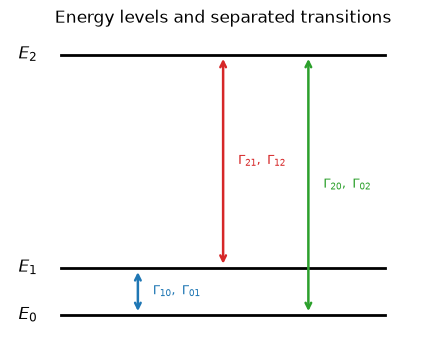
\includegraphics[width=0.5\textwidth]{screenshot001}
	\caption{}
	\label{fig:screenshot001}
\end{figure}
	
	A simple way to verify it is to construct a three-level classical systems .Define the prossibility matrix with Gibbs distribution
	\begin{equation}
	P_i(T)=\frac{ e^{-\frac{ E_i}{T}}}{ \sum_j e^{-\frac{ E_j}{T}}}
	\end{equation}
	  
	\begin{figure}[H]
		\centering
		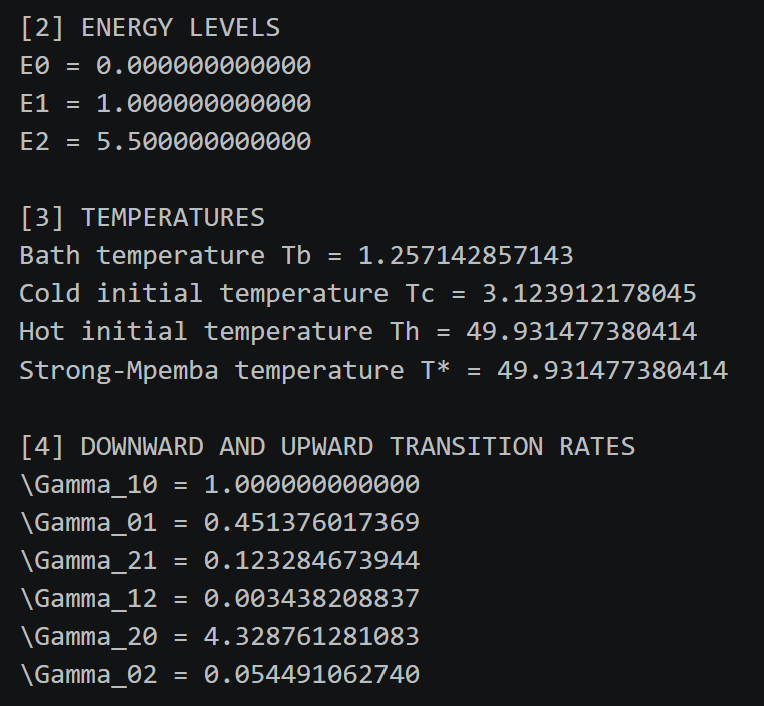
\includegraphics[width=0.35\textwidth]{screenshot005}
		\caption{}
		\label{fig:screenshot005}
	\end{figure}
 \begin{equation}
 	\label{eq:transition_matrix}
 	W =
 	\begin{pmatrix}
 		-\left(\Gamma_{01}+\Gamma_{02}\right)
 		& \Gamma_{10}
 		& \Gamma_{20}
 		\\[2mm]
 		\Gamma_{01}
 		& -\left(\Gamma_{10}+\Gamma_{12}\right)
 		& \Gamma_{21}
 		\\[2mm]
 		\Gamma_{02}
 		& \Gamma_{12}
 		& -\left(\Gamma_{20}+\Gamma_{21}\right)
 	\end{pmatrix}.
 \end{equation}
 We select the numerical values satisfying detailed balancing condition.
 \begin{equation}
 	\Gamma_{ij}P_{i}^{eq}=\Gamma_{ji}P_{j}^{eq}
  \end{equation}
 
 
	\begin{figure}[H]
		\centering
		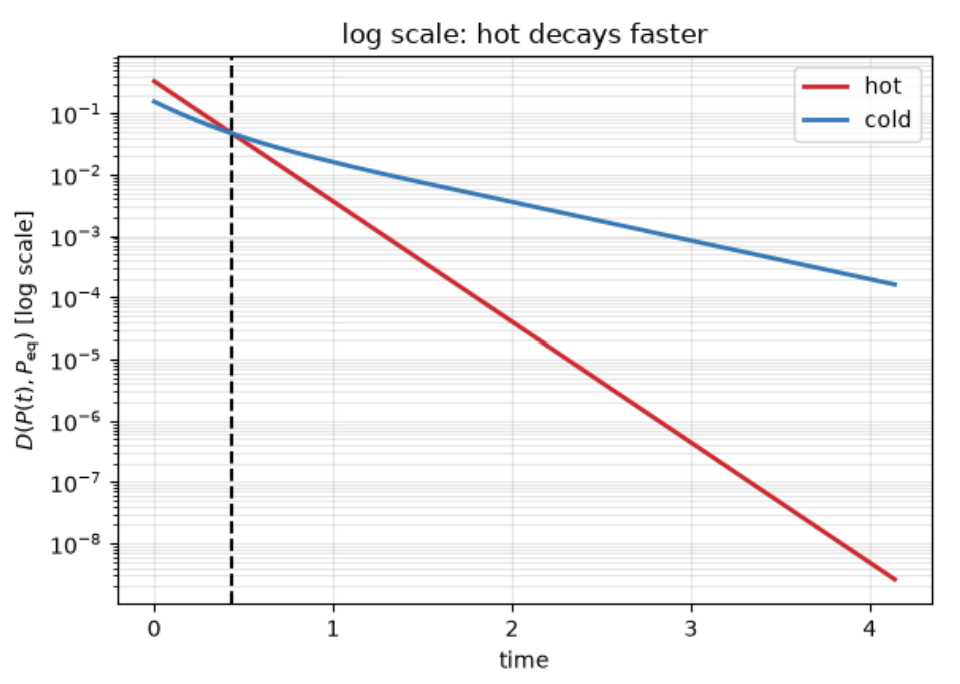
\includegraphics[width=0.5\textwidth]{screenshot004}
		\caption{}
		\label{fig:screenshot004}
	\end{figure}
	
 \begin{figure}[H]
 	\centering
 	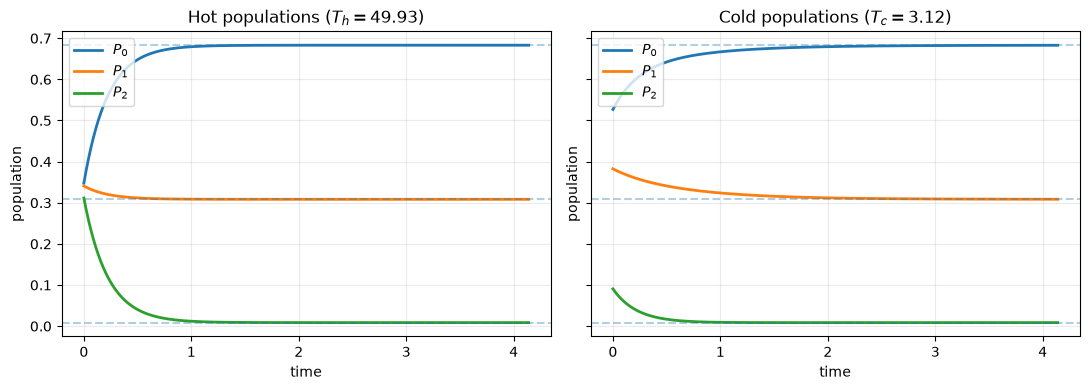
\includegraphics[width=0.5\textwidth]{screenshot003}
 	\caption{}
 	\label{fig:screenshot003}
 \end{figure}
 \section{ quantum Mpemba effect(example in closed system)}
   To study the Quantum Mpemba Effect (QME) more intuitively, we focus on the non-equilibrium dynamics of closed quantum systems. The traditional Mpemba effect typically concerns open systems coupled to an external environment, where states with different initial temperatures relax toward the same thermal equilibrium state; the anomaly lies in the fact that a state initially further from the final equilibrium can reach it sooner. The situation differs in closed quantum systems: there is no exchange of energy or information with the environment, and the system undergoes unitary evolution governed by
 
 $$ |\psi(t)\rangle=e^{-iHt}|\psi(0)\rangle $$
 
 Consequently, the Mpemba effect cannot be simply defined by the time required for a system to dissipate into a final equilibrium state. Instead, we examine the restoration of local symmetry. We begin by preparing a series of "tilted ferromagnetic states" with varying tilt angles, representing different degrees of broken $U(1)$ spin-rotation symmetry inherent in the Hamiltonian. Following a quantum quench, although the closed system as a whole evolves unitarily, its subsystems can undergo local relaxation and gradually restore this symmetry. In this context, the QME manifests as follows: a state with a greater initial degree of symmetry breaking achieves local symmetry restoration faster than a state with a lesser degree of breaking.
 We focus on XY model with attached field in z direction.
\begin{equation}
	H = \sum_{i<j}\frac{J_{ij}}{2}\left(\sigma_i^x\sigma_j^x+\sigma_i^y\sigma_j^y\right)
	+ \sum_i h_i\sigma_i^z
\end{equation}
 For the paper, the **tilted ferromagnetic state** can be written very explicitly as a tensor-product state.
 
 Starting from the fully polarized state,
 
 $$
 |\uparrow\uparrow\cdots\uparrow\rangle
 =
 |\uparrow\rangle^{\otimes N},
 $$
 
 rotate every spin by the same polar angle \(\theta\) and azimuthal angle \(\phi\).   Define  it as
 
 $$
 |TF(\theta,\phi)\rangle
 =
 e^{-i\phi \hat M_z}
 e^{-i\theta \hat M_y}
 |\uparrow\rangle^{\otimes N}.
 $$
 
 
 
 
 
 
 Therefore,
 
 $$
 	|TF(\theta,\phi)\rangle
 	=
 	\bigotimes_{j=1}^{N}
 	\left(
 	\cos\frac{\theta}{2}|\uparrow\rangle_j
 	+
 	e^{i\phi}\sin\frac{\theta}{2}|\downarrow\rangle_j
 	\right).
 $$
 
 For the case   \(\phi=0\),
 
 $$
 	|TF(\theta,0)\rangle
 	=
 	\left(
 	\cos\frac{\theta}{2}|\uparrow\rangle
 	+
 	\sin\frac{\theta}{2}|\downarrow\rangle
 	\right)^{\otimes N}.
 $$
 
 
 
for a subsystem A,
 We define the entanglement asymmetry 
 \begin{equation}
 	\Delta S_{A}=ln(Tr_{A}({\rho_A}^2))-ln(Tr_{A}({\rho_{\tilde{A}}}^2))
 \end{equation}
 
 where $\rho_{\tilde{A}}$is defined as $\sum_m \prod_m \rho \prod_m$
 $\prod_m$is the projection operator of eigenspace of $M_{z}^{A}$with eigenvalue m .EA describes how the titled state deviates from U(1)symmetry .EA vanishes only if $[\rho_A,M_{z}^{A}]=0$
 
 \begin{figure}[H]
 	\centering
 	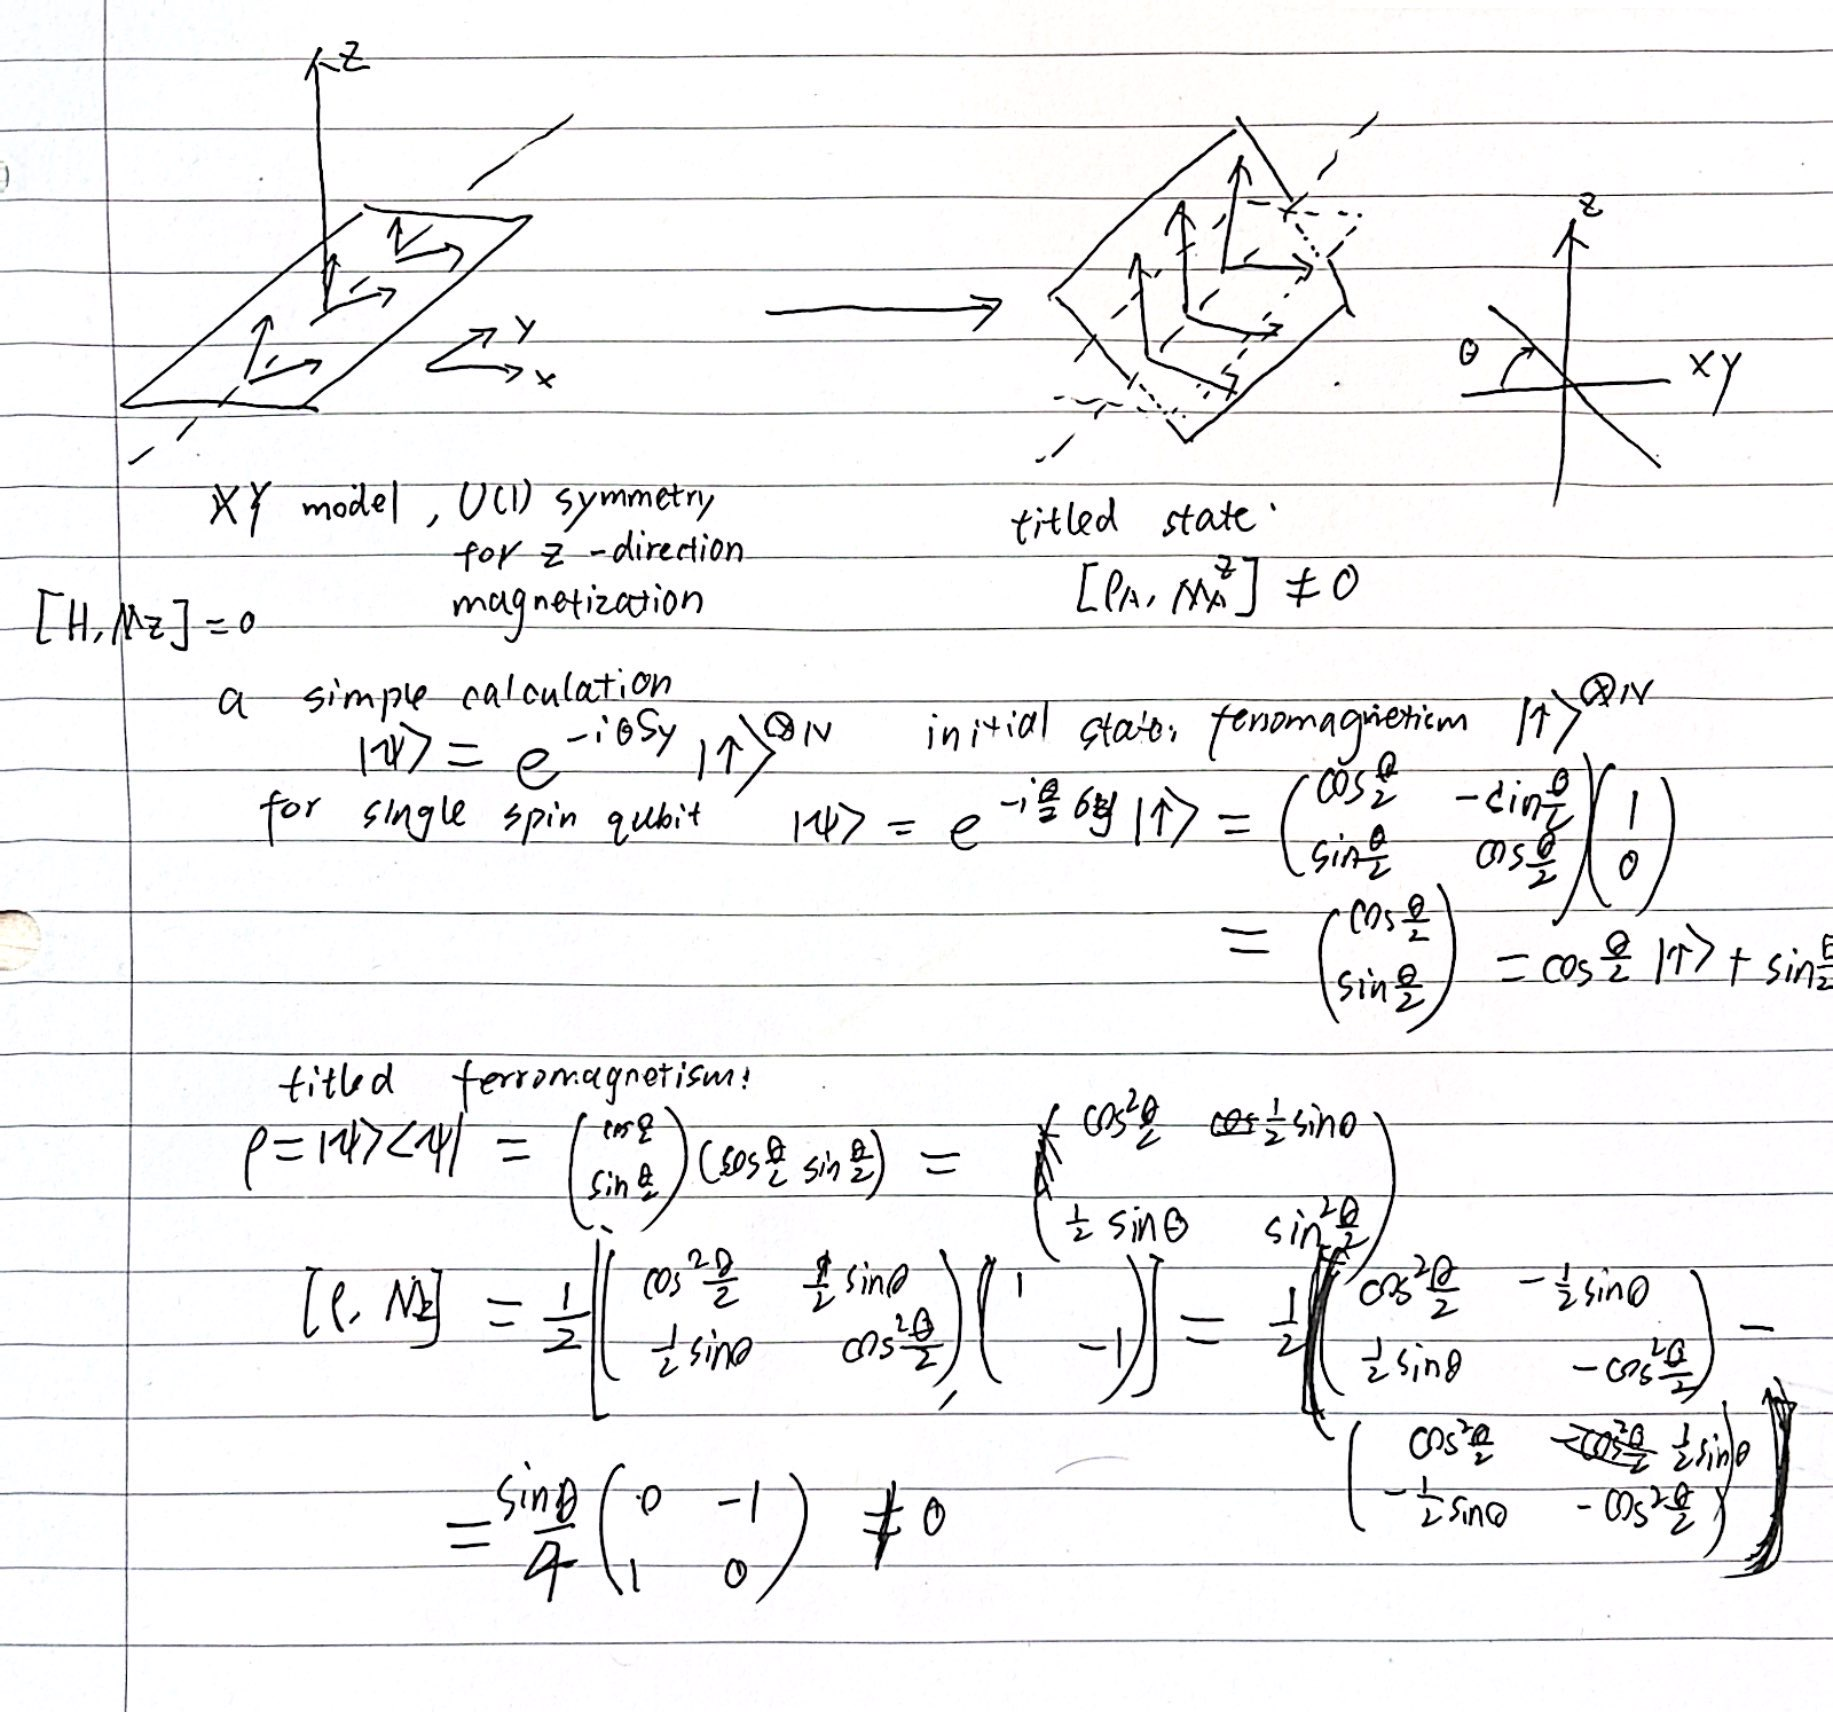
\includegraphics[width=1.0\linewidth]{Weixin Image_20260911133309_320_7.jpg}
		\caption{simple demonstration of the intial state and titled state.The direction of magnetization for the latter is rotated in Bloch sphere  }
 \end{figure}
  
	 \subsection{  macroscopic simulations  }
 
	  \subsubsection{power law  coupling  }
	 \begin{figure}[H]
	 	\centering
	 	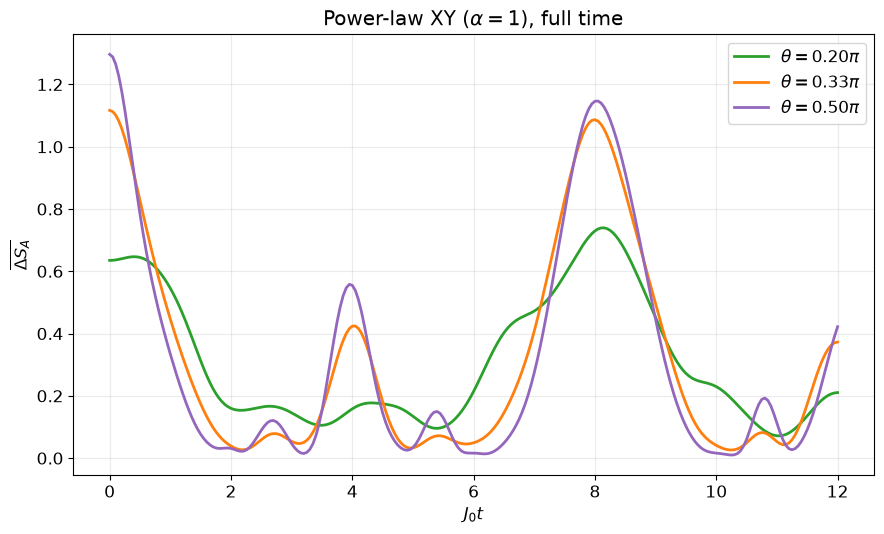
\includegraphics[width=1.0\linewidth]{screenshot007}
	 	\caption{The dynamics of EA.Because the evolution is unitary,different lines will cross and converge for many times.We only cares about the stage (0-3$J_0$t)}
	 	\label{fig:screenshot007}
	 \end{figure}
 
	 \begin{figure}[H]
	 	\centering
	 	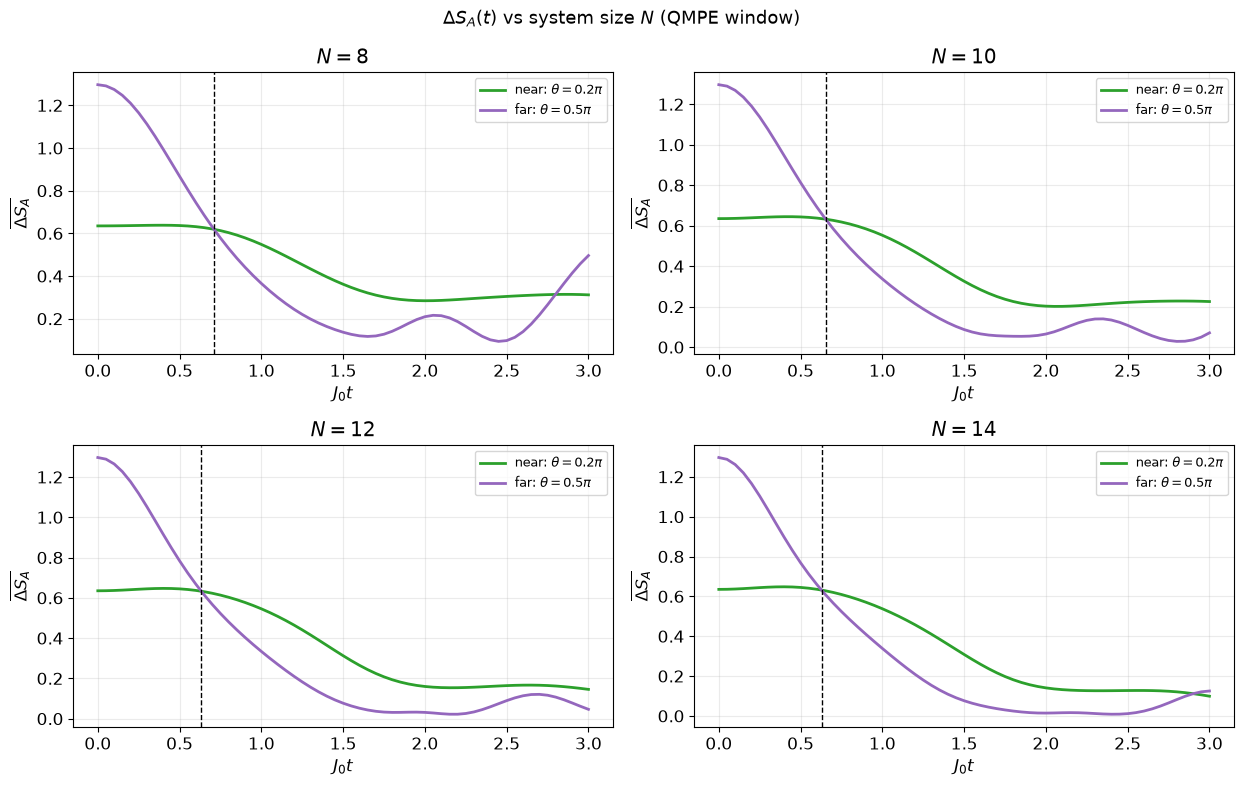
\includegraphics[width=1.0\linewidth]{screenshot016}
	 	\caption{exclude the finite-size effct}
	 	\label{fig:screenshot016}
	 \end{figure}
	 
	 \begin{figure}[H]
	 	\centering
	 	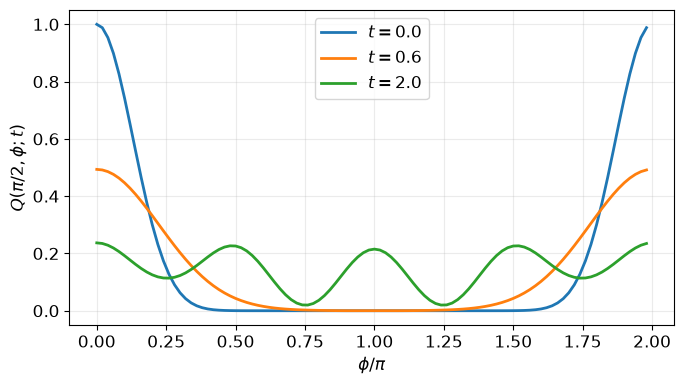
\includegraphics[width=1.0\linewidth]{screenshot012}
	 	\caption{N=12 chain.As the symmetry getting restored,
	 		the differences in angular distribution have been smoothed out.  }
	 	\label{fig:screenshot012}
	 \end{figure}
\begin{figure}[H]
	\centering
	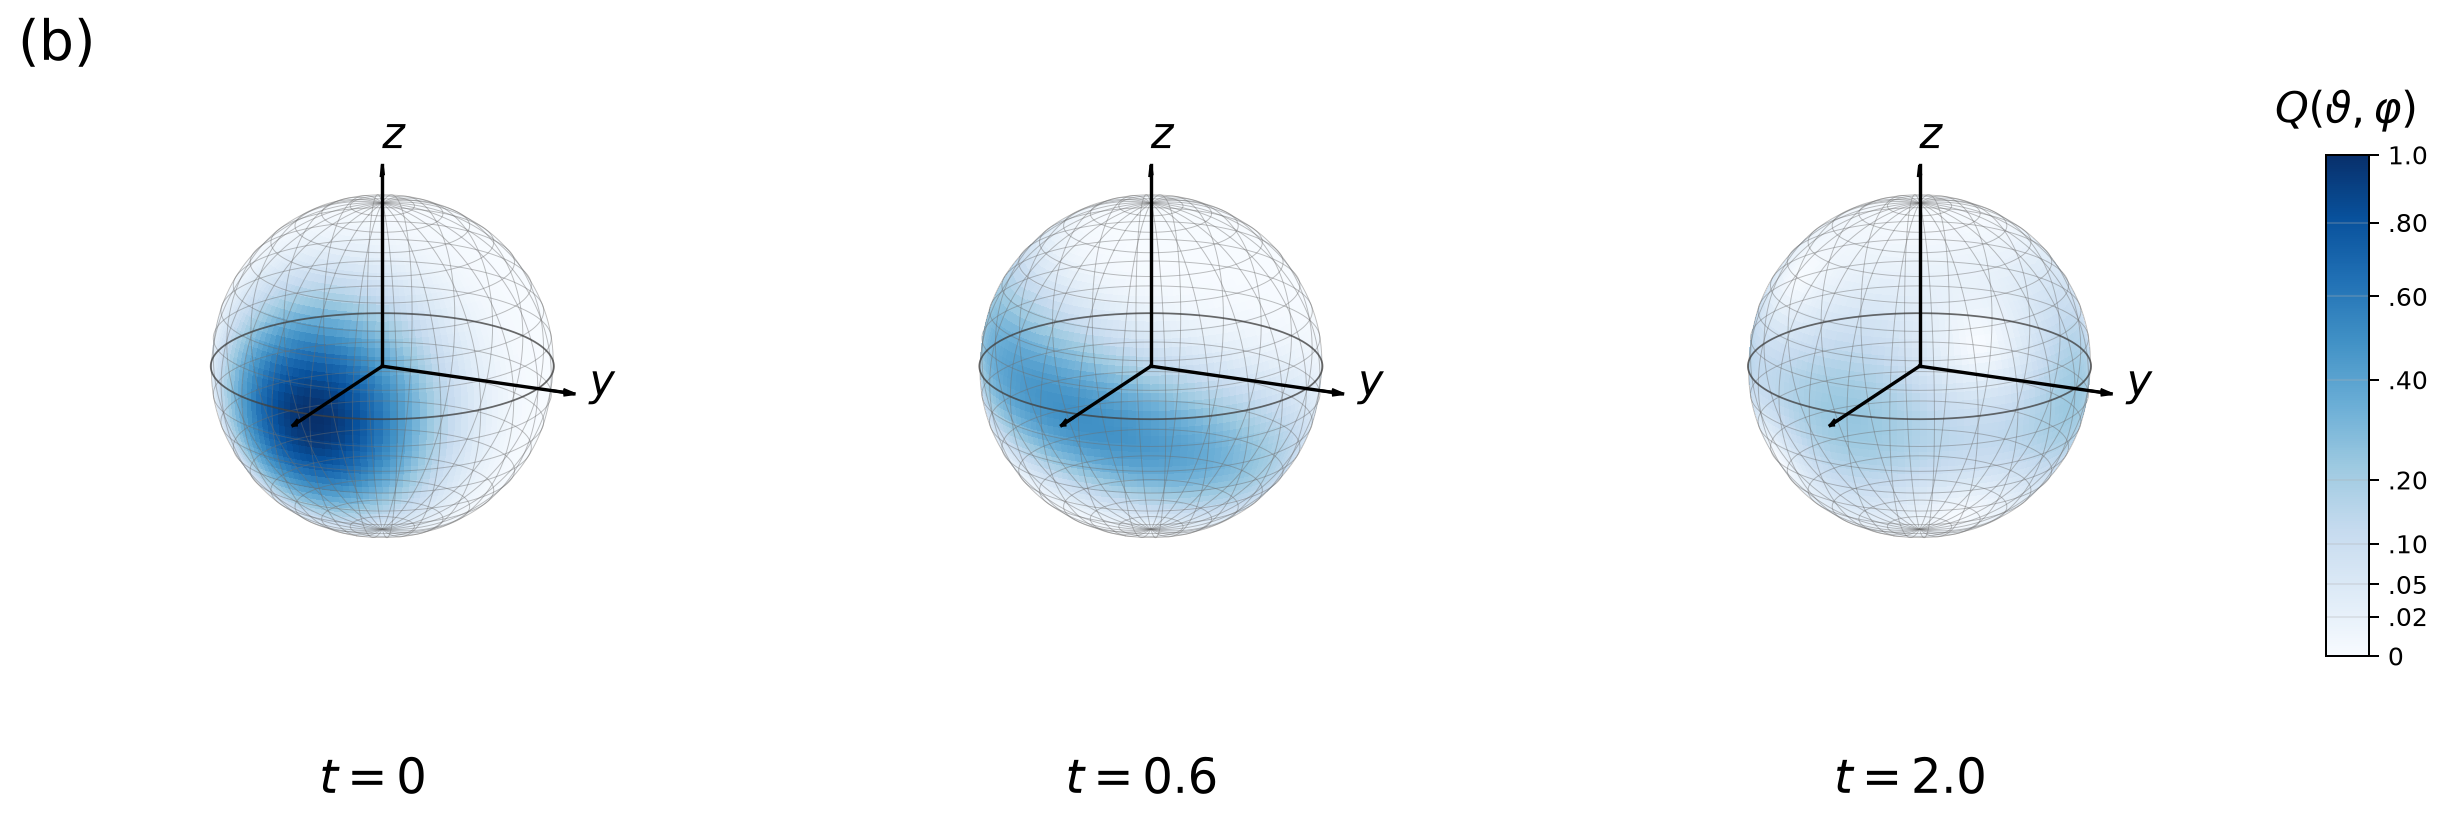
\includegraphics[width=1.0\linewidth]{screenshot014}
	\caption{ $Q(\phi,\theta)$is defined as the overlap between evoluted state and initial state }
	\label{fig:screenshot014}
\end{figure}
	 \begin{figure}[H]
	 	\centering
	 	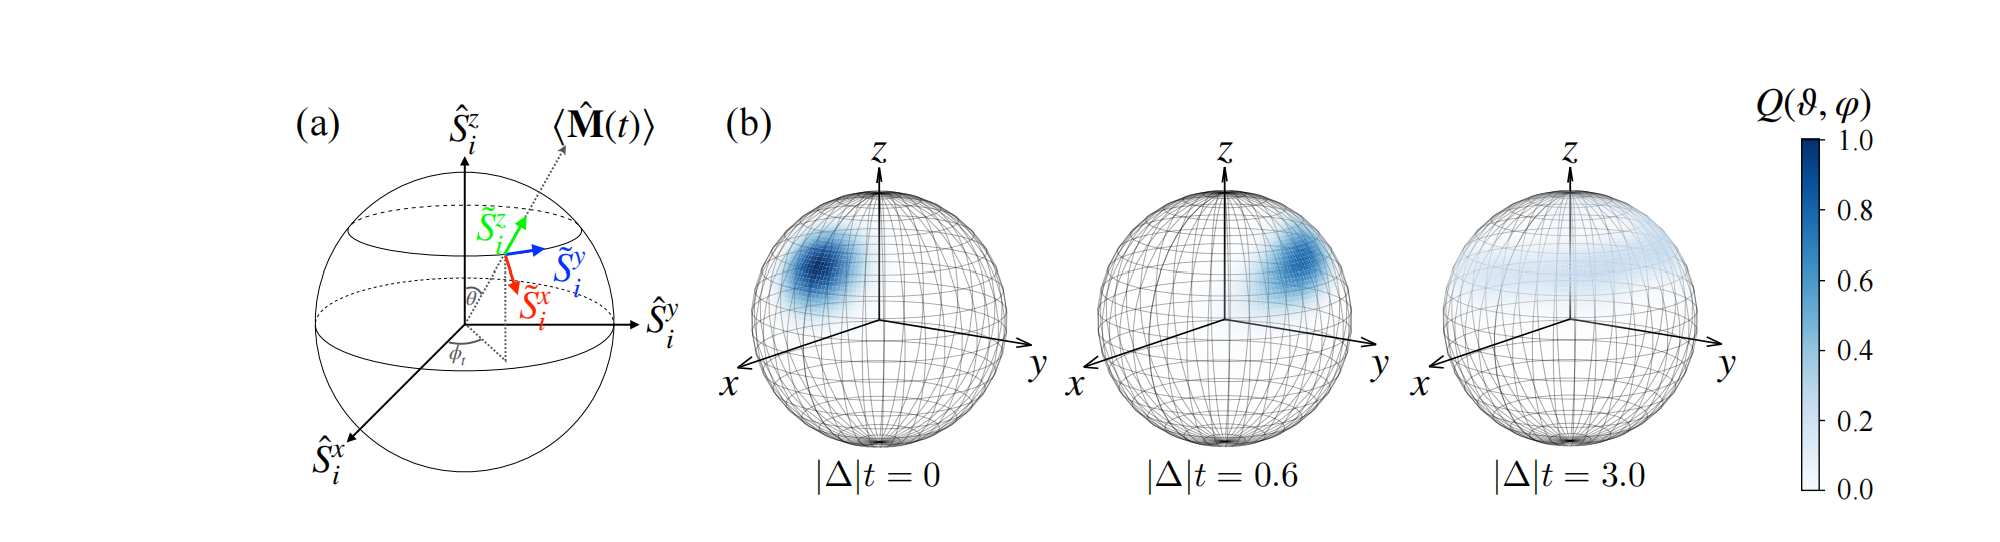
\includegraphics[width=1.0\linewidth]{screenshot015}
	 	\caption{ideal figure }
	 	\label{fig:screenshot015}
	 \end{figure}
	 
	 
	 \begin{figure}[H]
	 	\centering
	 	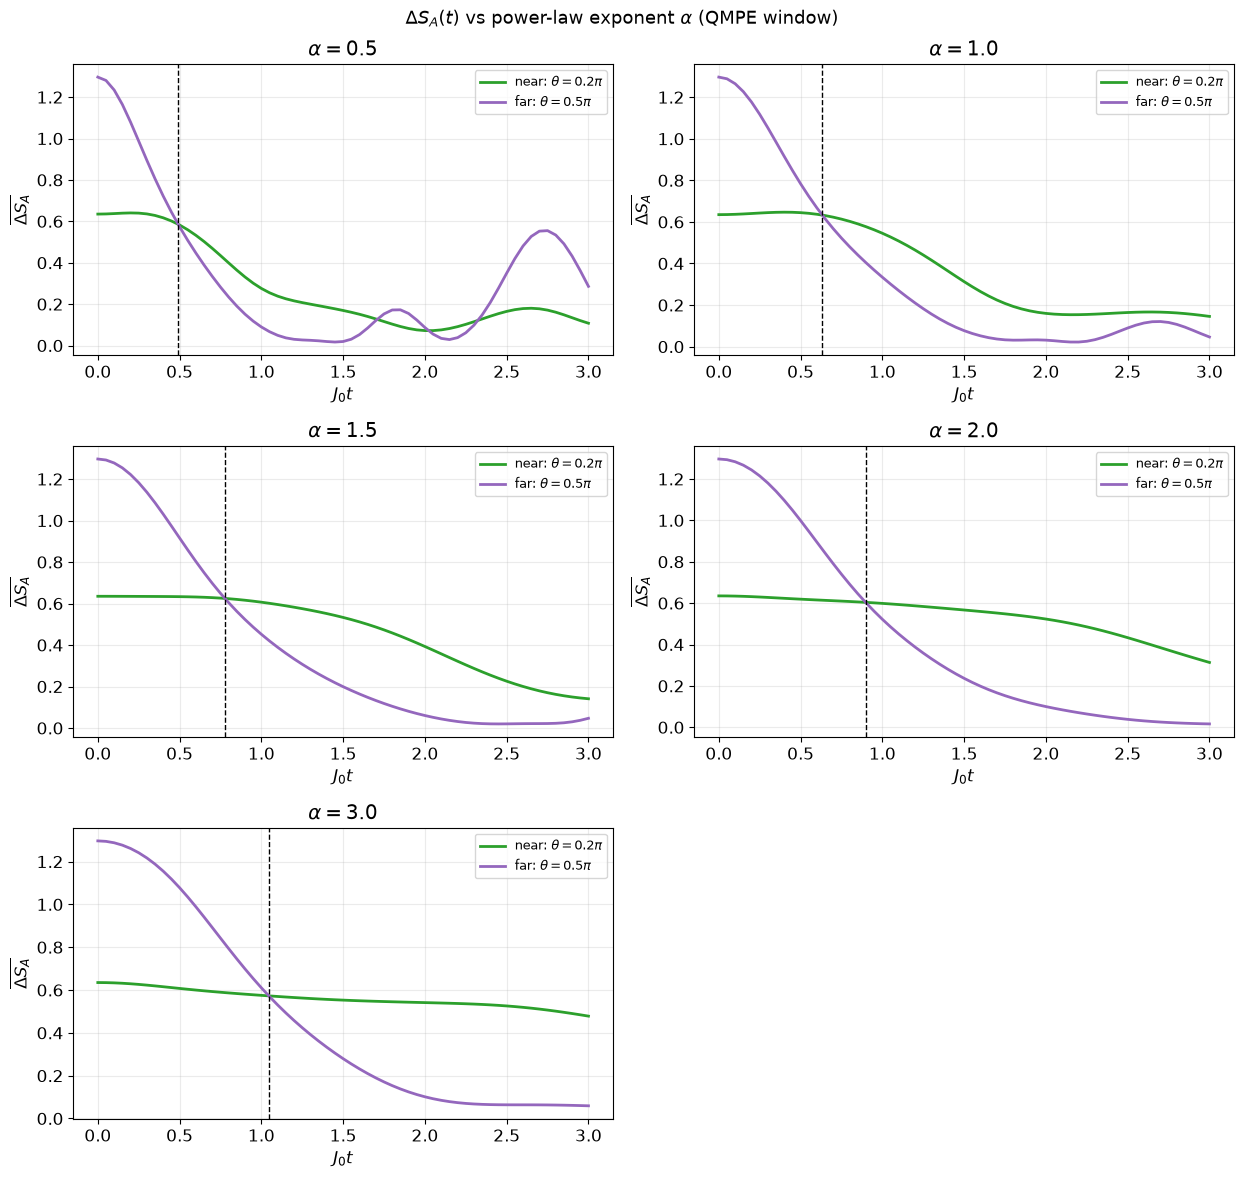
\includegraphics[width=1.0\linewidth]{screenshot006}
	 	\caption{EA(t) with different power-law exponent $\alpha$}
	 	\label{fig:screenshot006}
	 \end{figure}
	 
	 
	 
	 \subsubsection{exponential decaying coupling  }
	 \begin{figure}[H]
	 	\centering
	 	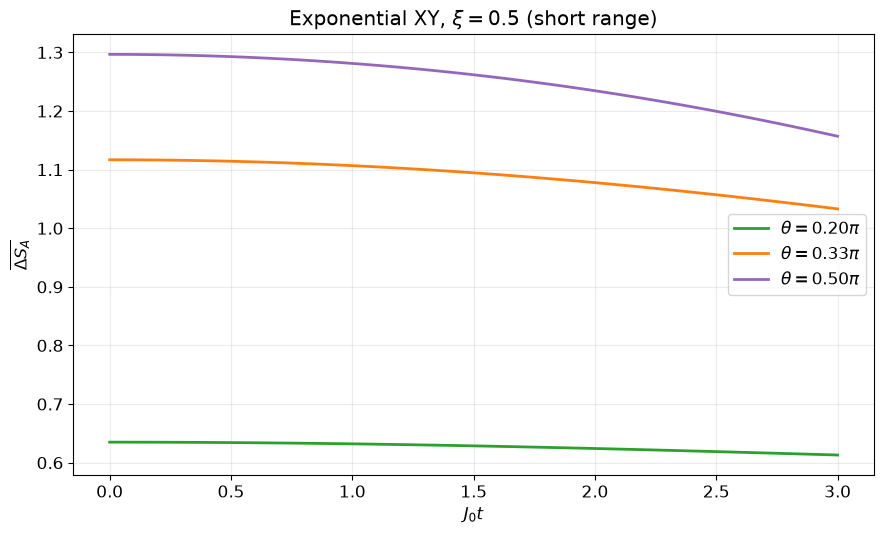
\includegraphics[width=1.0\linewidth]{screenshot008}
	 	\caption{for$\xi$=0.5 case,we do not observe QME in finite time }
	 	\label{fig:screenshot008}
	 \end{figure}
	 \begin{figure}[H]
	 	\centering
	 	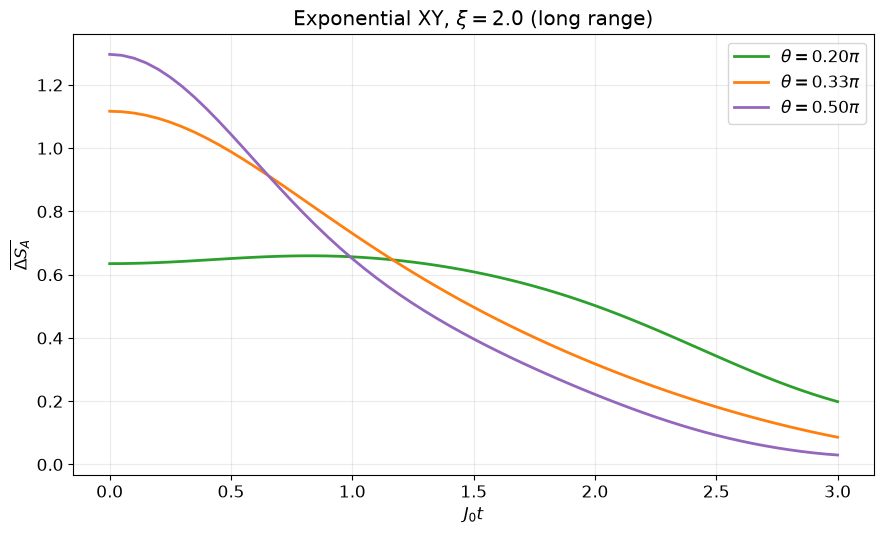
\includegraphics[width=1.0\linewidth]{screenshot009}
	 	\caption{for $\xi=2$ case,QME comes back unexpectedly}
	 	\label{fig:screenshot009}
	 \end{figure}
	 \begin{figure}[H]
	 	\centering
	 	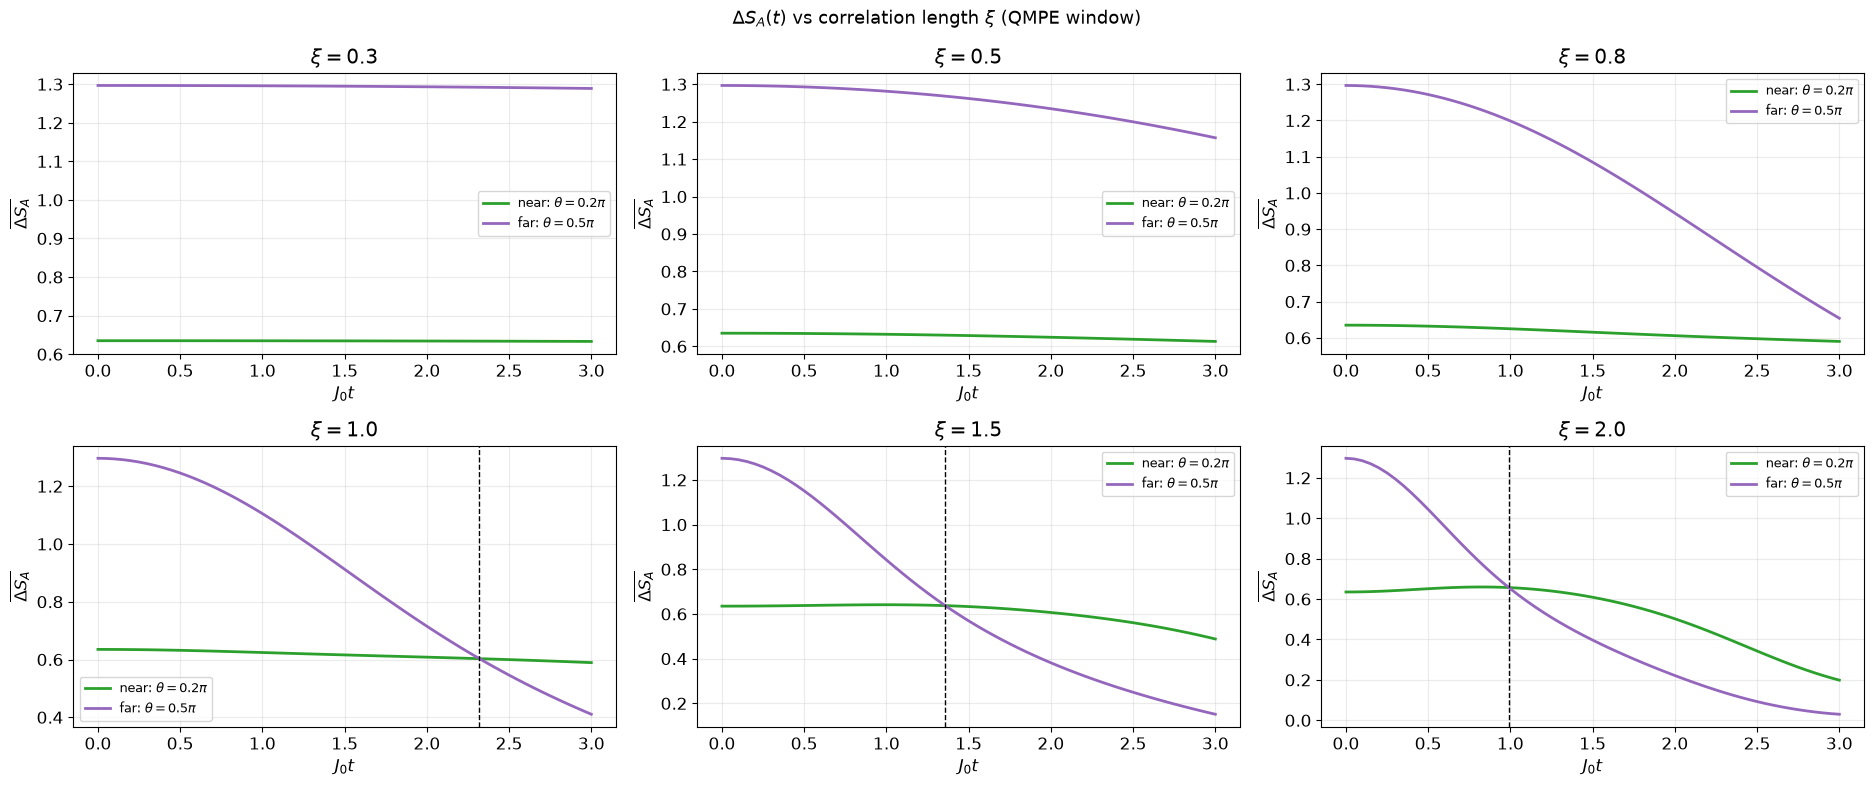
\includegraphics[width=1.0\linewidth]{screenshot010}
	 	\caption{As the characteristic length increases,QME comes back and the crossing time is moved up  }
	 	\label{fig:screenshot010}
	 \end{figure}
	  For QME in short range interaction systems,there are some different interpretations such as charge transport picture.
	 \subsubsection{ disorder }
	 \begin{figure}[H]
	 	\centering
	 	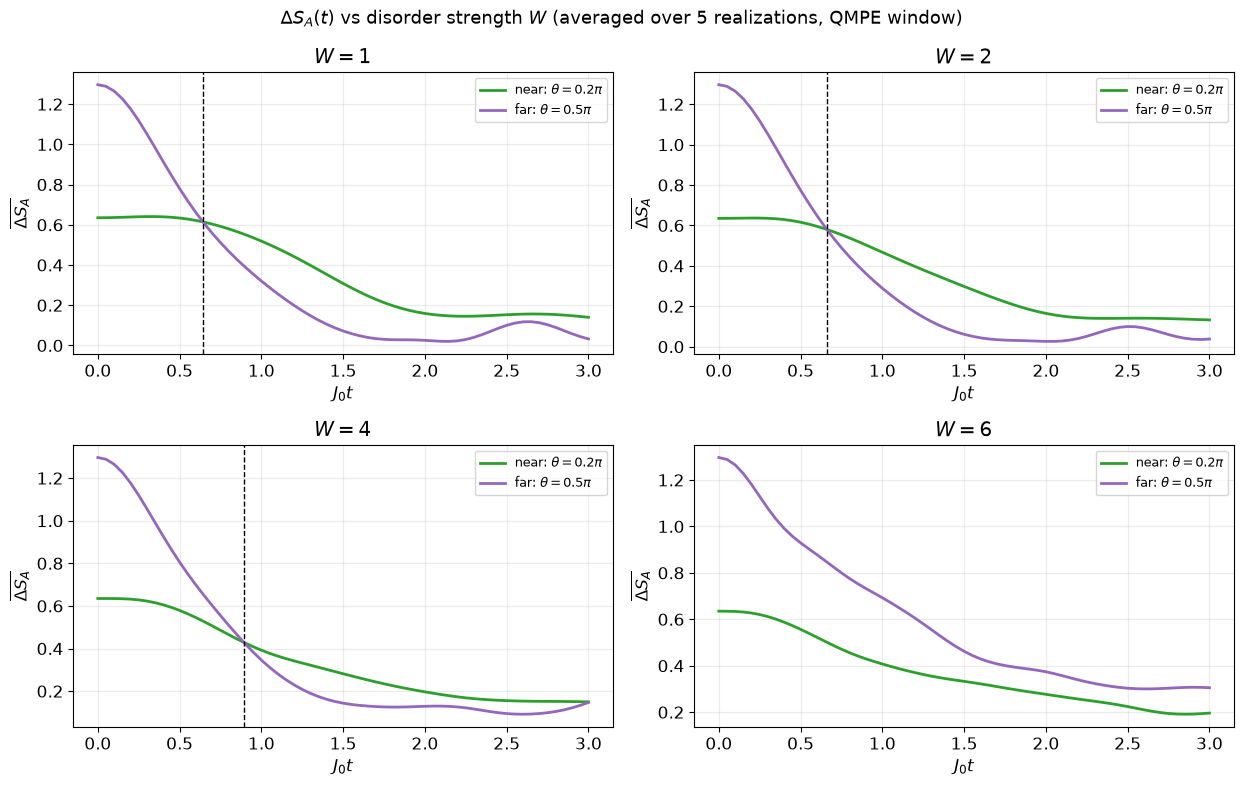
\includegraphics[width=1.0\linewidth]{screenshot011}
	 	\caption{disorder in the z direction destroys QME}
	 	\label{fig:screenshot011}
	 \end{figure}
		 \subsubsection{ Gradient-ordered potential}
		 
		 \subsection{ microscopic picture:how and why ? }	
	 
		 \subsubsection{quantum fluctuations and dissipation} 
		 	 \subsection{from closed system to open systems!Where is new physics?}
		 	 for long-range model
		 	 By HP transformation in the rotated frame ,
		 	 the initial tilted-ferromagnetic state corresponds to the
		 	 bosonic vacuum state, and the quantum fluctuations of
		 	 spins are described by bosonic excitations, which are referred to as spin waves.
		\section{Appendix}	
		\subsection{ theoretical frame for long range coupling systems}
		 
		To describe the fluctuations, the authors introduce a  rotating frame  whose \(\tilde z\)-axis follows the instantaneous magnetization \(\langle\mathbf M(t)\rangle\). In this frame, the large classical motion of the magnetization is separated from the quantum fluctuations around it. The Holstein–Primakoff transformation then maps these small transverse spin fluctuations onto bosonic excitations, or spin waves,
		
		$$
		\tilde S_i^x\simeq
		\sqrt{\frac{s}{2}}(b_i+b_i^\dagger),\qquad
		\tilde S_i^y\simeq
		i\sqrt{\frac{s}{2}}(b_i^\dagger-b_i),\qquad\\
		\tilde S_i^z=s-b_i^\dagger b_i .
		$$
		\begin{figure}[H]
			\centering
			\includegraphics[width=1.0\linewidth]{"Weixin Image_20260913121340_328_7"}
			\caption{}
			\label{fig:weixin-image202609131213403287}
		\end{figure}
		
		
		In this description, the initial tilted ferromagnetic state corresponds to the bosonic vacuum, while spin waves generated during the time evolution represent quantum fluctuations around the collective magnetization. 
		
		Keeping the Hamiltonian only up to quadratic order in the bosonic operators gives
		
		$$
		\tilde H\simeq
		\frac{1}{2s}\sum_k
		\left(
		\xi_k b_k^\dagger b_k
		+
		\kappa_k b_k^\dagger b_{-k}^\dagger
		+\mathrm{H.c.}
		\right),
		$$
		
		with
		
		$$
		\kappa_k=\tilde J_k\Delta\sin^2\theta .
		$$
		
		The important term is
		
		$$
		\kappa_k b_k^\dagger b_{-k}^\dagger,
		$$
		
		because it creates pairs of spin waves with momenta \(k\) and \(-k\) from the initial bosonic vacuum. Therefore, \(\kappa_k\) controls the generation of quantum fluctuations. Since
		
		$$
		\kappa_k\propto\sin^2\theta,
		$$
		
		a state with a larger initial tilt angle generally generates stronger spin-wave fluctuations. 
		
		The corresponding occupation of the \(k\)-th spin-wave mode is
		
		$$
		n_k(t)
		=
		\frac{\Delta^2\tilde J_k^2\sin^4\theta}{\omega_k^2}
		\sin^2\left(\frac{\omega_k t}{s}\right),
		$$
		
		where
		
		$$
		\omega_k=\sqrt{\xi_k^2-\kappa_k^2}.
		$$
		
		Thus, the production of spin-wave fluctuations has a strong dependence on the initial tilt through the factor \(\sin^4\theta\). 
		
		For the restoration of the \(U(1)\) symmetry, the most important contribution comes from the zero-momentum mode \(k=0\). The entanglement asymmetry can be approximated by
		
		$$
		\Delta S_A(t)
		\simeq
		\frac12
		\ln
		\left[
		\frac{
			2s\pi N_A\sin^2\theta
		}{
			1+4n_0(t)f_A(1-f_A)
		}
		\right],
		\qquad
		f_A=\frac{N_A}{N}.
		$$
		
		Therefore, as \(n_0(t)\) increases, the entanglement asymmetry decreases:
		
		$$
		n_0(t)\uparrow
		\quad\Rightarrow\quad
		\Delta S_A(t)\downarrow.
		$$
		
		Since \(\Delta S_A=0\) corresponds to the restoration of the local \(U(1)\) symmetry, the zero-momentum spin waves directly drive the symmetry-restoration process. 
		
		The physical meaning of \(n_0\) becomes clearer by expressing it in terms of fluctuations of the total magnetization in the rotating frame,
		
		$$
		n_0=
		\frac{
			\operatorname{Var}(\tilde M^x)
			+
			\operatorname{Var}(\tilde M^y)
		}{2sN}
		-\frac12 .
		$$
		
		The authors show that the fluctuation that grows during the evolution is mainly the azimuthal component,
		
		$$
		\operatorname{Var}(\tilde M^y).
		$$
		
		Therefore, the direction of the collective magnetization becomes increasingly uncertain along the azimuthal angle \(\phi\). Since the original tilted ferromagnetic state breaks the \(U(1)\) symmetry by selecting a particular azimuthal direction, spreading the quantum state along \(\phi\) progressively removes this preferred direction and restores the rotational symmetry around the laboratory \(z\)-axis. 
		
		The theoretical origin of the QME can therefore be summarized as
		
		$$
		\theta\uparrow
		\;\Rightarrow\;
		\kappa_0\propto\sin^2\theta\uparrow
		\;\Rightarrow\;
		n_0(t)\text{ grows faster}
		\;\Rightarrow\;
		\text{azimuthal quantum fluctuations grow faster}
		$$
		
		$$
		\Rightarrow\;
		\Delta S_A(t)\text{ decreases faster}
		\;\Rightarrow\;
		U(1)\text{ symmetry is restored faster}.
		$$
		
		Hence, the initially more strongly tilted state, although it breaks the \(U(1)\) symmetry more strongly, generates collective quantum fluctuations more rapidly and consequently restores the symmetry sooner. This provides the microscopic spin-wave explanation of the Quantum Mpemba Effect in the article.  	 
 \end{document}